\documentclass[12pt]{article}

\usepackage[utf8]{inputenc}
\usepackage{fancyhdr}
\usepackage{xcolor,graphicx}
\usepackage{fancyvrb}
\usepackage{tcolorbox}
\usepackage{hyperref}
\hypersetup{
    colorlinks=true,
    linkcolor=blue,
    filecolor=blue,      
    urlcolor=blue,
}

% Allow explicit linebreaks in table items
\usepackage{makecell}
\usepackage{float}

% Allow tables to span page boundaries.
\usepackage{longtable}
\setlength{\LTpre}{5pt}
\setlength{\LTpost}{5pt}

\pagestyle{fancy}

%\lhead{Parallel Computing with LMGC90}
\chead{}
\rhead{} 
\lfoot{}
\cfoot{}
\rfoot{\hfill \thepage}
\renewcommand{\headrulewidth}{0pt}

\fancypagestyle{mypagestyle}{%
\lhead{}
\chead{}
\rhead{} 
\lfoot{}
\cfoot{}
\rfoot{\hfill \thepage}
}

% No indent text 
\setlength\parindent{0pt}
\setlength\parskip{1mm plus 1mm}

% Space between paragraphs
\setlength{\parskip}{2.0\parskip}

%%%%%%%%%%%%%%%%%%%%%%%%%%%%%%%%%%%%%%%%%%%%%
%%%%%%%%%%%%%%%%%%%%%%%%%%%%%%%%%%%%%%%%%%%%%
%%%%%%%%%%%%%%%%%%%%%%%%%%%%%%%%%%%%%%%%%%%%%

\begin{document}

\thispagestyle{mypagestyle}

\begin{center}
  \textbf{\Large Installing LMGC90 on Cedar and Graham Compute Canada servers}\\
  \today
\end{center}

\section*{Disclaimers}
\textbf{If} you need to learn how to access ComputeCanada, how servers are structured or how to upload and download data on clusters, we recommend that you refer to our original instruction manual or the inexhaustible source of information \href{https://docs.computecanada.ca/wiki/Compute_Canada_Documentation}{\underline{ComputeCanada\_wiki}}.

\textbf{If} you plan to use Béluga or Niagara, we also recommend that you refer to the previous notice which will give you exhaustive instructions to install LMGC90 and start learning its use on clusters.\hfill \\
\rule{\linewidth}{.5pt}

\textbf{If} you plan to use Cedar or Graham, follow the instructions below.\\
\textbf{NOTE1:} If you never worked on ComputeCanada servers with LMGC90, we advise you to begin with small steps on Béluga.\\
\textbf{NOTE2:} Use one of the version of LMGC90 available on the \href{https://git-xen.lmgc.univ-montp2.fr/lmgc90/lmgc90_user/-/wikis/download_and_install}{\underline{website}}.\hfill \vspace{0.5cm}
ComputeCanada is the national network of servers for high-performance computing. It is composed of 4 main servers:
\begin{itemize}
    \item Cedar
    \item Graham
    \item Béluga
    \item Niagara
\end{itemize}

Each one of them is provided a set of modules which allow you to switch between different versions of software packages you may want to use. This root set is called a “standard environment” and is named \texttt{StdEnv}. At the present time it exists three competing versions of these \texttt{2016.4}, \texttt{2018.3} and \texttt{2020}. For those of you who might want to investigate what truly lies behind, learn that detailed information on the major additions developed between each version can be find \href{https://docs.computecanada.ca/wiki/Standard_software_environments}{\underline{here}}.

\texttt{StdEnv/2016.4} is the standard environment originally implemented on both Cedar and Graham. It explains why the implementations of LMGC90 on those clusters needs a different handling procedure.  

\section*{Modules in the server}
First and foremost, we remind you that at any time and in any repertory of your server share you can access to the list of modules loaded by using the command:

\begin{tcolorbox}
\texttt{[name@server $\sim$]\$ module list}
\end{tcolorbox}

By doing so you must obtain an initial structure similar to this one:
\begin{figure}[H]
  \centering
  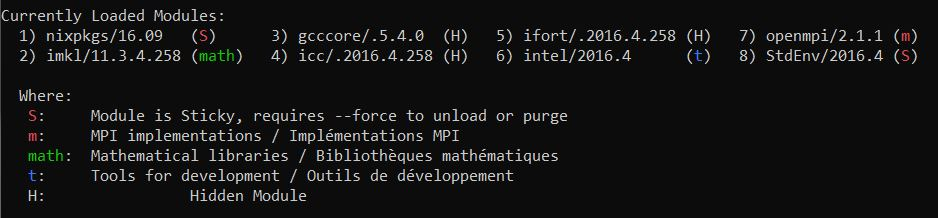
\includegraphics[width=1.\linewidth]{Screen1.jpg}
\end{figure}
\textbf{NOTE:} If it is not the case, do not worry and stick to the following instructions.

At this point, you need to have uploaded LMGC90 data in a definite folder in such location:
\begin{tcolorbox}
\texttt{[name@server $\sim$]\$ cd projects/account\_name/name/lmgc90\_ folder/}
\end{tcolorbox}
\textbf{NOTE:} If you need to get your location, don’t forget to use the command:
\begin{tcolorbox}
\texttt{[name@server $\sim$]\$ pwd}\\
\texttt{/the/corresponding/path/of/your/location}
\end{tcolorbox}
\vspace{1cm}
To load the modules that allow us to compile LMGC90, write the following line:
\begin{tcolorbox}
\texttt{[name@server lmgc90\_folder]\$ module purge \textcolor{red}{\textbf{A}}} 
\end{tcolorbox}
Now, understand that the compilation of LMGC90 requires specific modules but that the root set \texttt{StdEnv/2016.4} is unable to provide the proper versions of such material. In rare circumstances it may be then necessary to load a different standard environment to access particular versions of needed packages. We are actually looking for its next update named \texttt{StdEnv/2018.3} which you can load by overwriting the former environment:
\begin{tcolorbox}
\texttt{[name@server lmgc90\_folder]\$ module load StdEnv/2018.3 \textcolor{red}{\textbf{B}}} 
\end{tcolorbox}

\textbf{NOTE:} If the one above does not work, you may try:
\begin{tcolorbox}
\texttt{[name@server lmgc90\_folder]\$ module switch StdEnv/2016.4 StdEnv/2018.3 \textcolor{red}{\textbf{B*}}} 
\end{tcolorbox}
\begin{figure}[H]
  \centering
  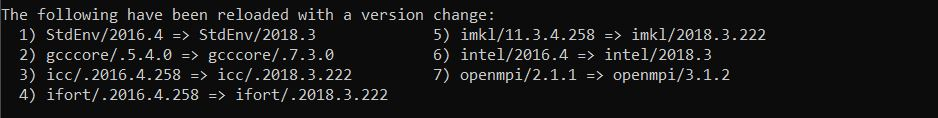
\includegraphics[width=1.\linewidth]{Screen2.jpg}
\end{figure}

Also, add:
\begin{tcolorbox}
\texttt{[name@server lmgc90\_folder]\$ module load vtk nixpkgs/16.09 gcc/7.3.0 hdf5 \textcolor{red}{\textbf{C}}} 
\end{tcolorbox}
\begin{figure}[H]
  \centering
  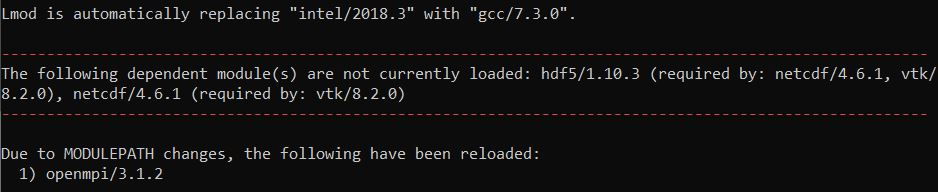
\includegraphics[width=1.\linewidth]{Screen3.jpg}
\end{figure}
\vspace{1cm}
Hopefully, you have obtained this type of response.
\begin{figure}[H]
  \centering
  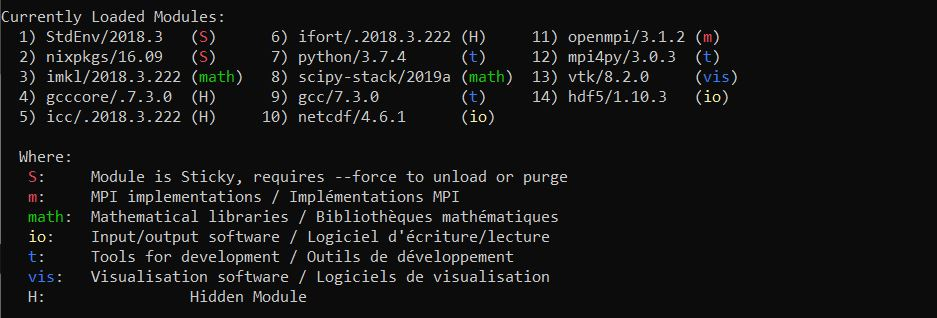
\includegraphics[width=1.\linewidth]{Screen4.jpg}
\end{figure}
You will need to run the same three lines \textcolor{red}{(\texttt{\textbf{A}}, \texttt{\textbf{B}} or \texttt{\textbf{B*}} and \texttt{\textbf{C}})} before running your simulations. In fact, you will systematically add them in each bash script from which we describe the structure later.

\section*{Installing LMGC90}

Adequate modules are now loaded. The compilation is done as explained below following the procedure given by the \href{https://git-xen.lmgc.univ-montp2.fr/lmgc90/lmgc90_user/-/wikis/Compilation}{\underline{LMGC90\_wiki page}}. 

Create a \texttt{build} folder with:
\begin{tcolorbox}
\texttt{[name@server lmgc90\_folder]\$ mkdir build} 
\end{tcolorbox}
Access to the \texttt{build}:
\begin{tcolorbox}
\texttt{[name@server lmgc90\_folder]\$ cd build}
\end{tcolorbox}
And compile with:
\begin{tcolorbox}
\texttt{[name@server build]\$ cmake .. -DMATLIB\_VERSION=none -DSPARSE\_LIBRARY=none} 
\end{tcolorbox}
\vspace{1.5cm}
Finally:
\begin{tcolorbox}
\texttt{[name@server build]\$ make} 
\end{tcolorbox}

The compilation went probably well, without raising any issue to your attention.

\section*{Running your simulations with the queuing assistant: SLURM}

You must use a queuing assistant called SLURM to run your simulations from one of the two clusters we are interested in.  We propose to work with a bash script. This same script will have to be in the folder of your simulation located somewhere in your \texttt{scratch}:
\begin{tcolorbox}
\texttt{[name@server $\sim$]\$ cd scratch/path/simu\_folder/}\\
\texttt{[name@server simu\_folder]\$ pwd}\\
\texttt{/home/name/scratch/path/simu\_folder}
\end{tcolorbox}

After you have uploaded the \texttt{DATBOX} folder and the \texttt{command.py} referring to your simulation in its folder, create the bash script with the command:
\begin{tcolorbox}
\texttt{[name@server simu\_folder]\$ nano script.sh} 
\end{tcolorbox}

In the nano editor you are then able to write a simple bash script from which we give you an example of structure below.
\begin{figure}[H]
  \centering
  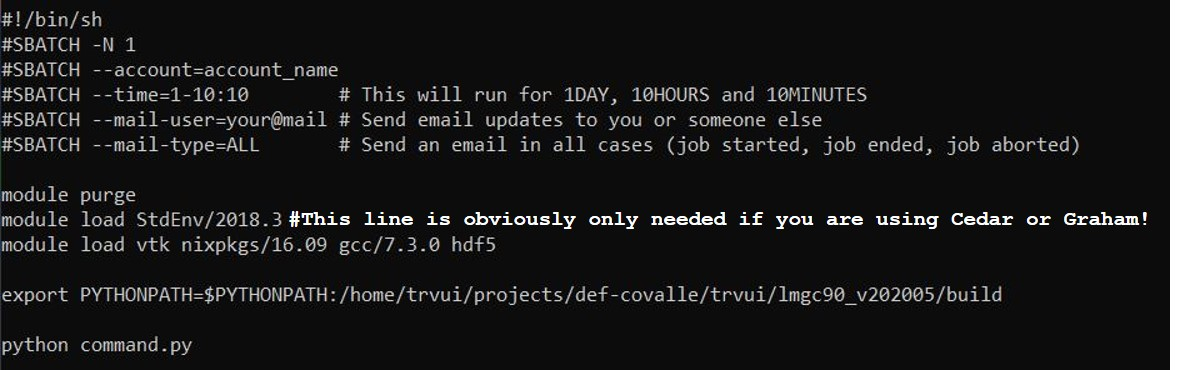
\includegraphics[width=1.\linewidth]{Screen5.jpg}
\end{figure}
\begin{itemize}
    \item The first line says that this is a bash script.
    \item Second line states that this belongs to the group \texttt{account\_name}.
    \item Third line states the duration of the simulation. In Cedar and Graham the limit is set to 28 days.
    \item Fourth and fifth lines are optional but helpful. They will keep you updated of your simulation’s state by email so you do not have to keep an eye on it constantly.
    \item Then, the modules are purged and loaded as required.
    \item Next line states where the sources of LMGC90 are located.
    \item And finally, we run the simulation.
\end{itemize} 

Then, run it using:
\begin{tcolorbox}
\texttt{[name@server simu\_folder]\$ sbatch script.sh}
\end{tcolorbox}

\textbf{NOTE:} If you want to learn more about the SLURM options, we recommend that you refer to the last chapter of our original instruction manual.


\end{document}